%%%%%%%%%%%%%%%%%%%%%%%%%%%%%%%%%%%%%%%%%%%%%%%%%%%%%%%%%%%%%%%%%%%%%%%%%%%%%%%%%%%%%%%%%%%%%
%%									ANNEXES 												%
%%%%%%%%%%%%%%%%%%%%%%%%%%%%%%%%%%%%%%%%%%%%%%%%%%%%%%%%%%%%%%%%%%%%%%%%%%%%%%%%%%%%%%%%%%%%%
\chapter{Annexes}

%%%%%%%%%%%%%%%%%%%%%%%%%%%%%%%%%%%%%%%%%%%%%%%%%%%%%%%%%%%%%%%%%%%%%%%%%%%%%%%%%%%%%%%%%%%%%


\section{Figures annexes}

\begin{figure}[!h]
	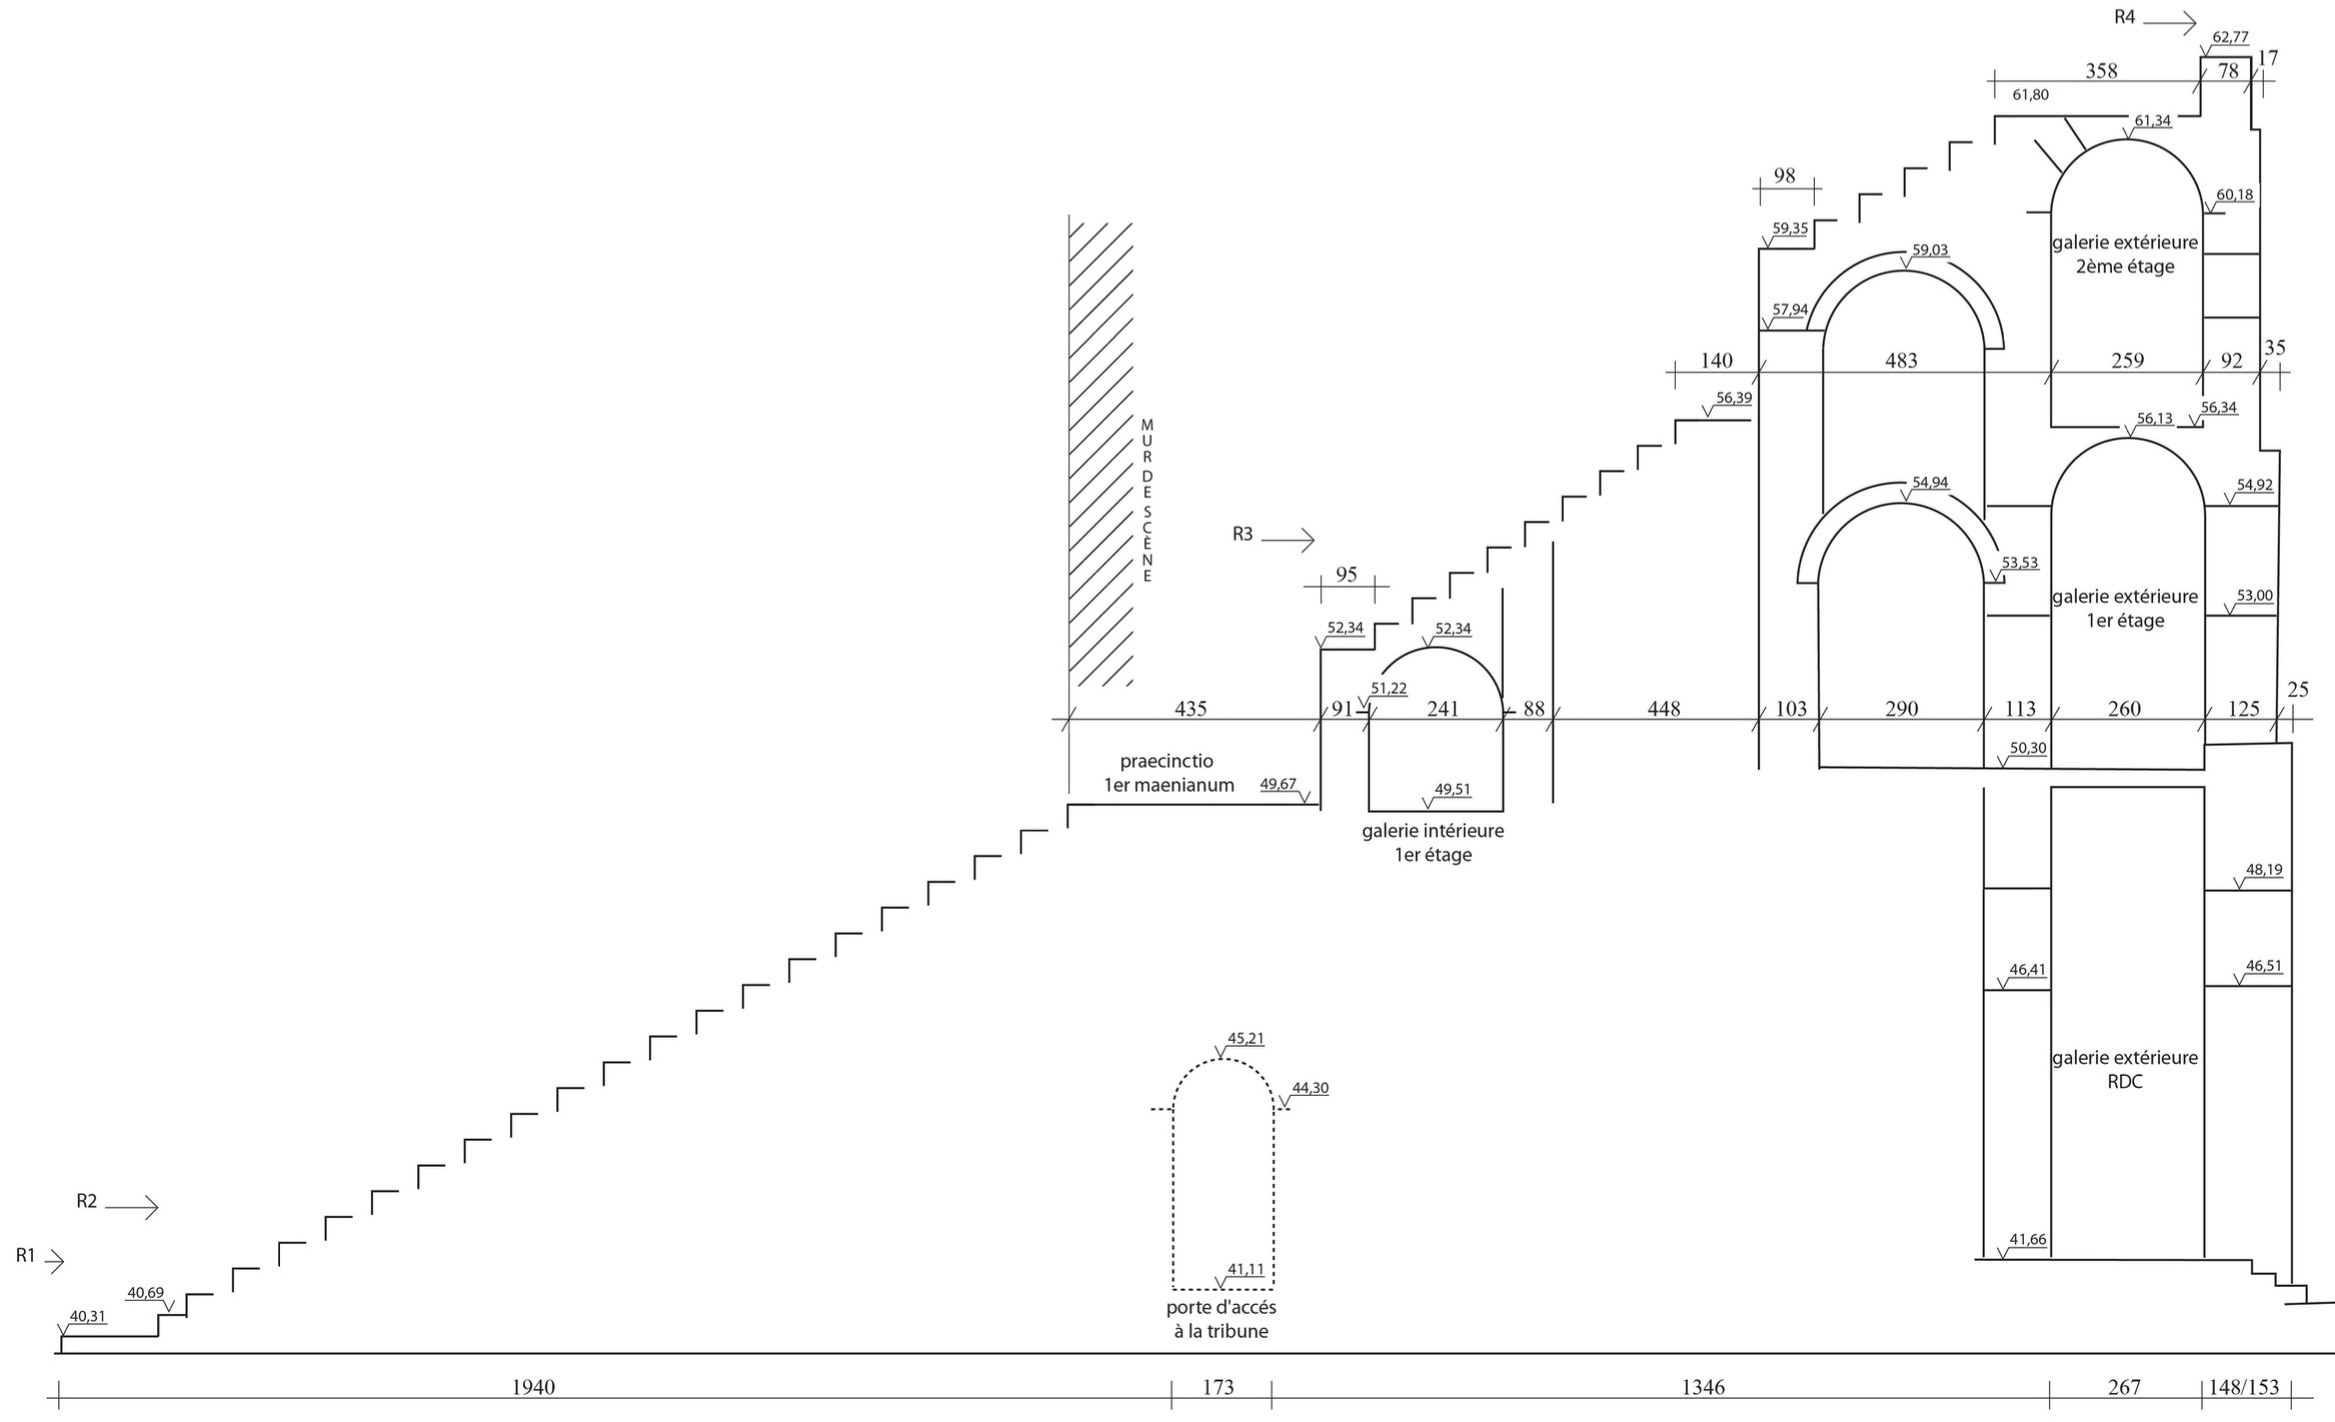
\includegraphics[width=\linewidth]{images/CoupeCavea}
	\caption[Coupe théorique sur la \gls{cavea}]{Coupe théorique sur la \gls{cavea} \cite[Pl. LX]{orangePl}} 
	\label{coupeCavea} 
\end{figure} 

\begin{figure}[!h]
	\includegraphics[width=\linewidth]{images/caristieDessus}
	\caption[Vue de dessus par A. Caristie 1856]{Représentation de l'état du théâtre d'Orange en 1856 en vue de dessus par A. Caristie \cite[Pl. I]{orangePl}} 
	\label{caristieDessus} 
\end{figure} 
	
\begin{figure}[!h]
	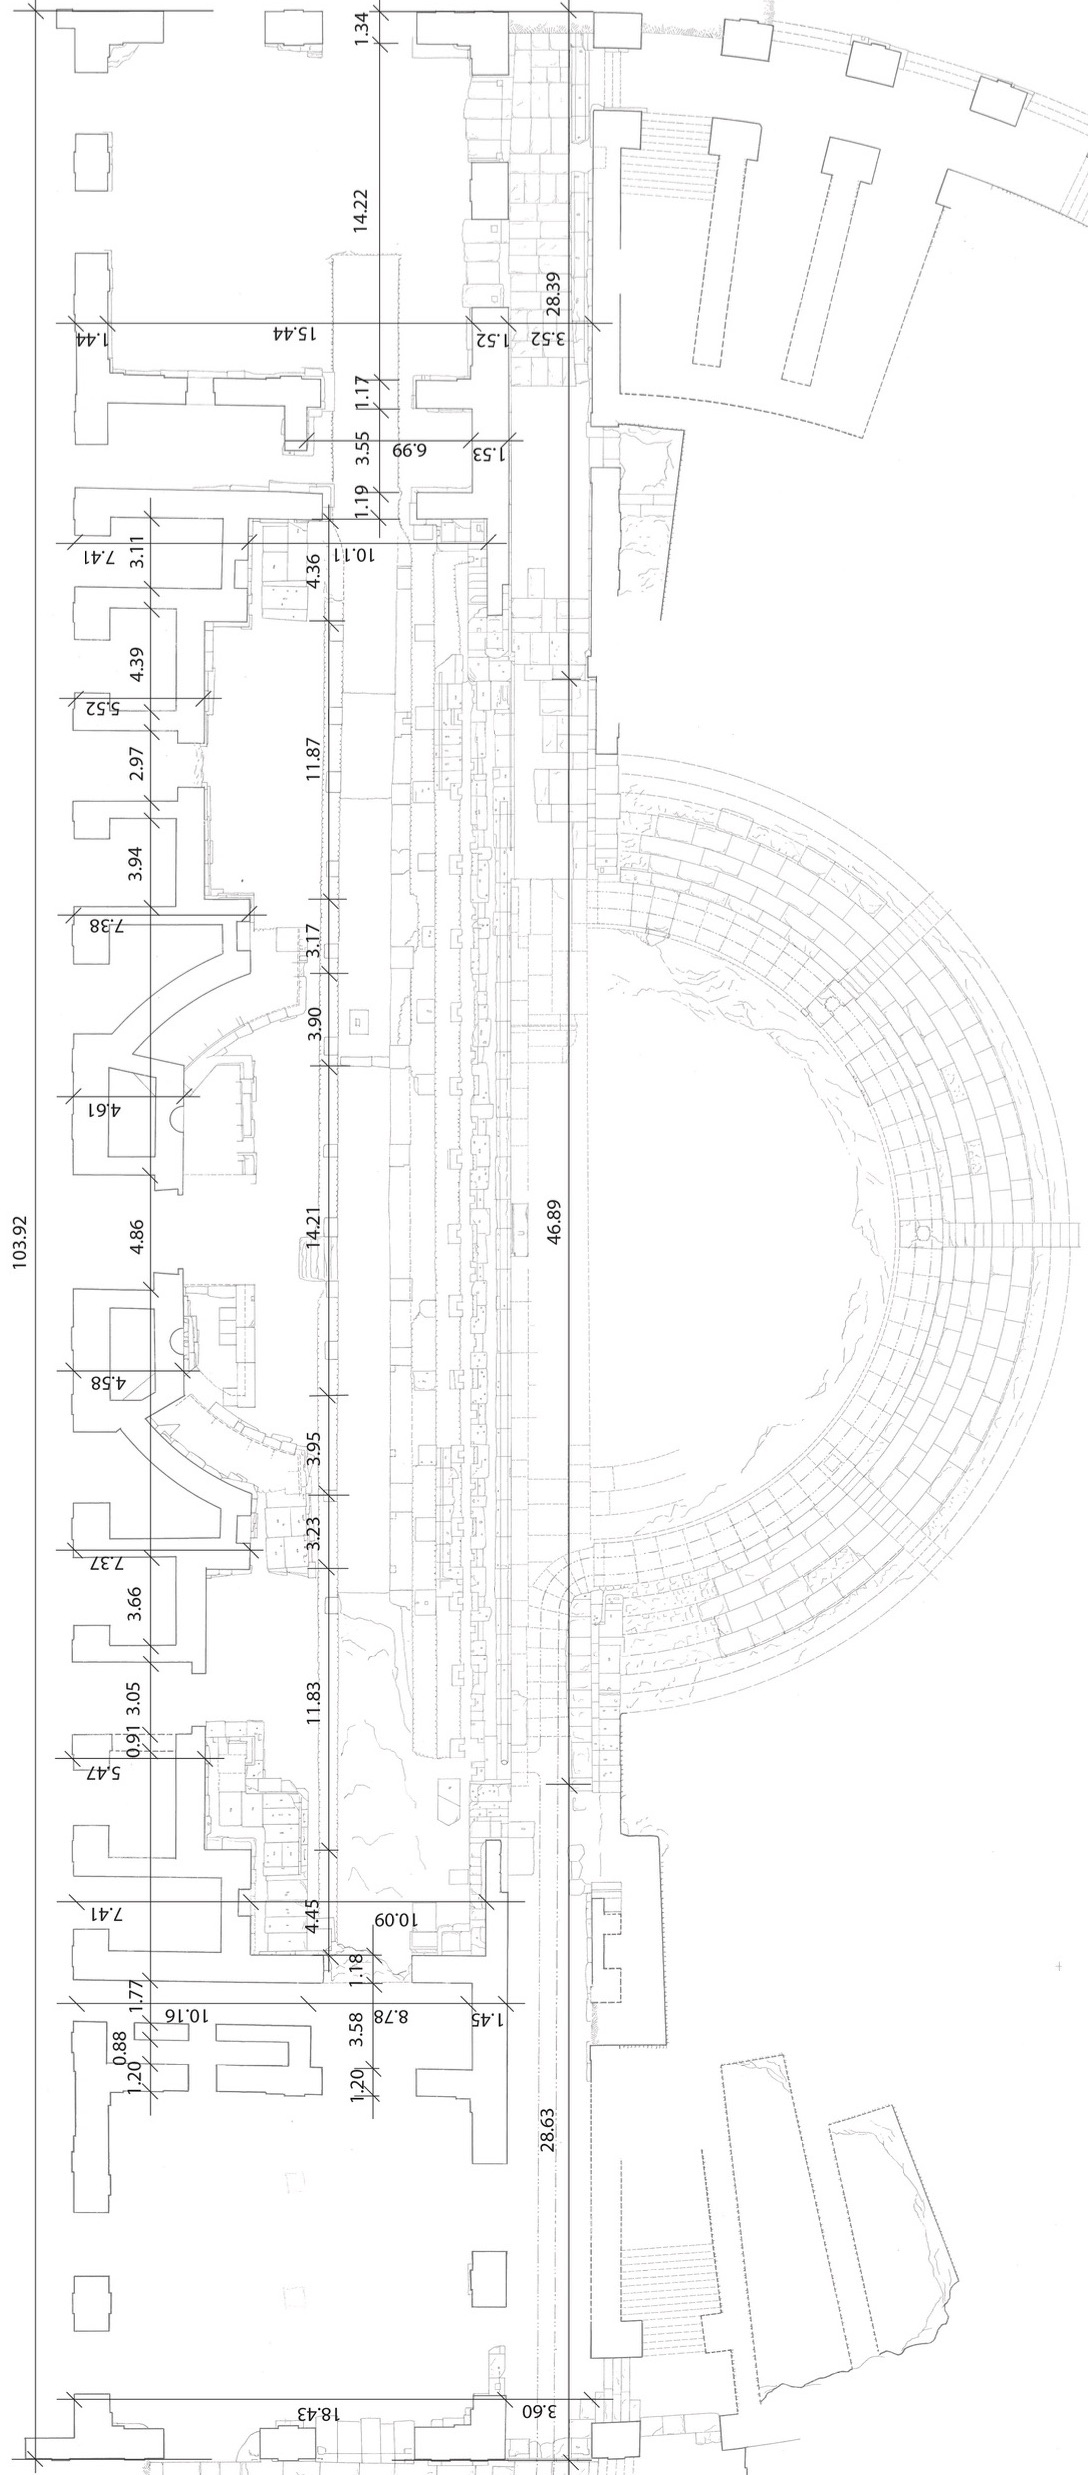
\includegraphics[height=0.8\paperheight]{images/cotes}
	\caption[Plan du rez-de-chaussée au bâtiment de scène]{Plan du rez-de-chaussée au bâtiment de scène \cite[Pl. XXI]{orangePl}}
	\label{cotes} 
\end{figure} 

\begin{figure}[!h]
		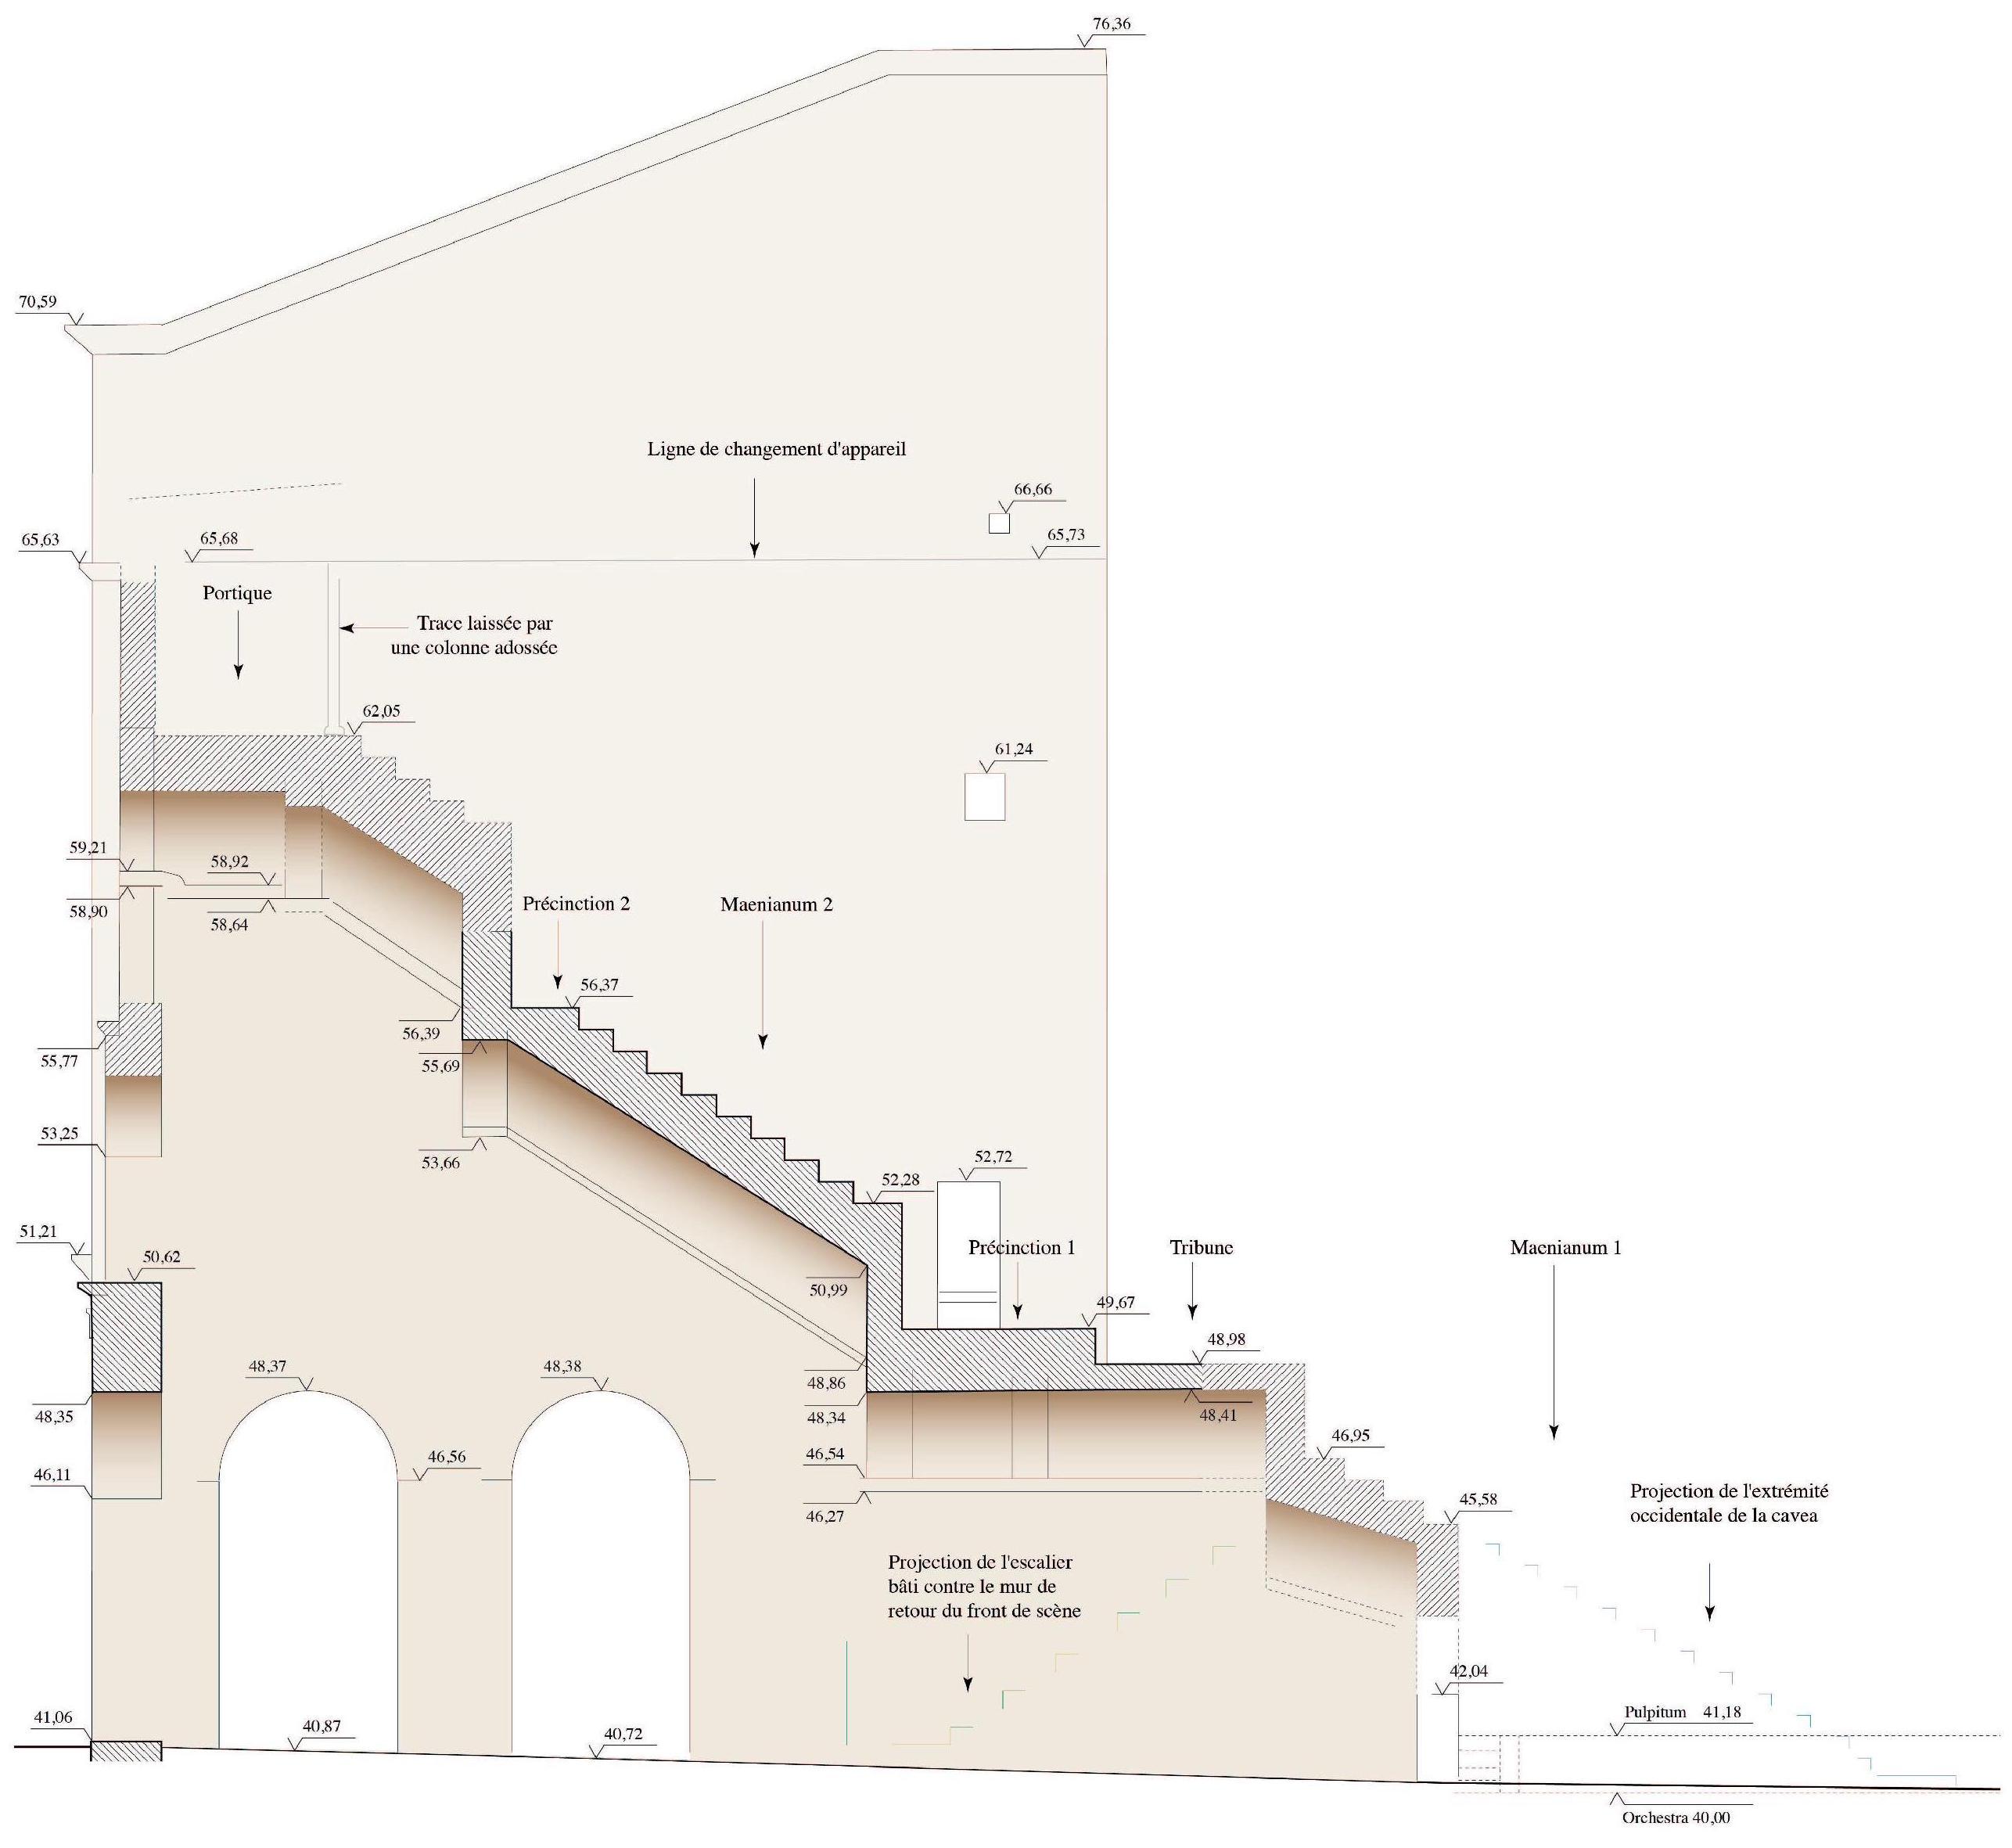
\includegraphics[width=\linewidth]{images/aditusOccidental}
		\caption[Coupe sur l'\gls{aditus} occidental]{Coupe sur l'\gls{aditus} occidental \cite[Pl. XLVIII]{orangePl}}
		\label{aditusOccidental}	
\end{figure}

\begin{figure}[!h]
		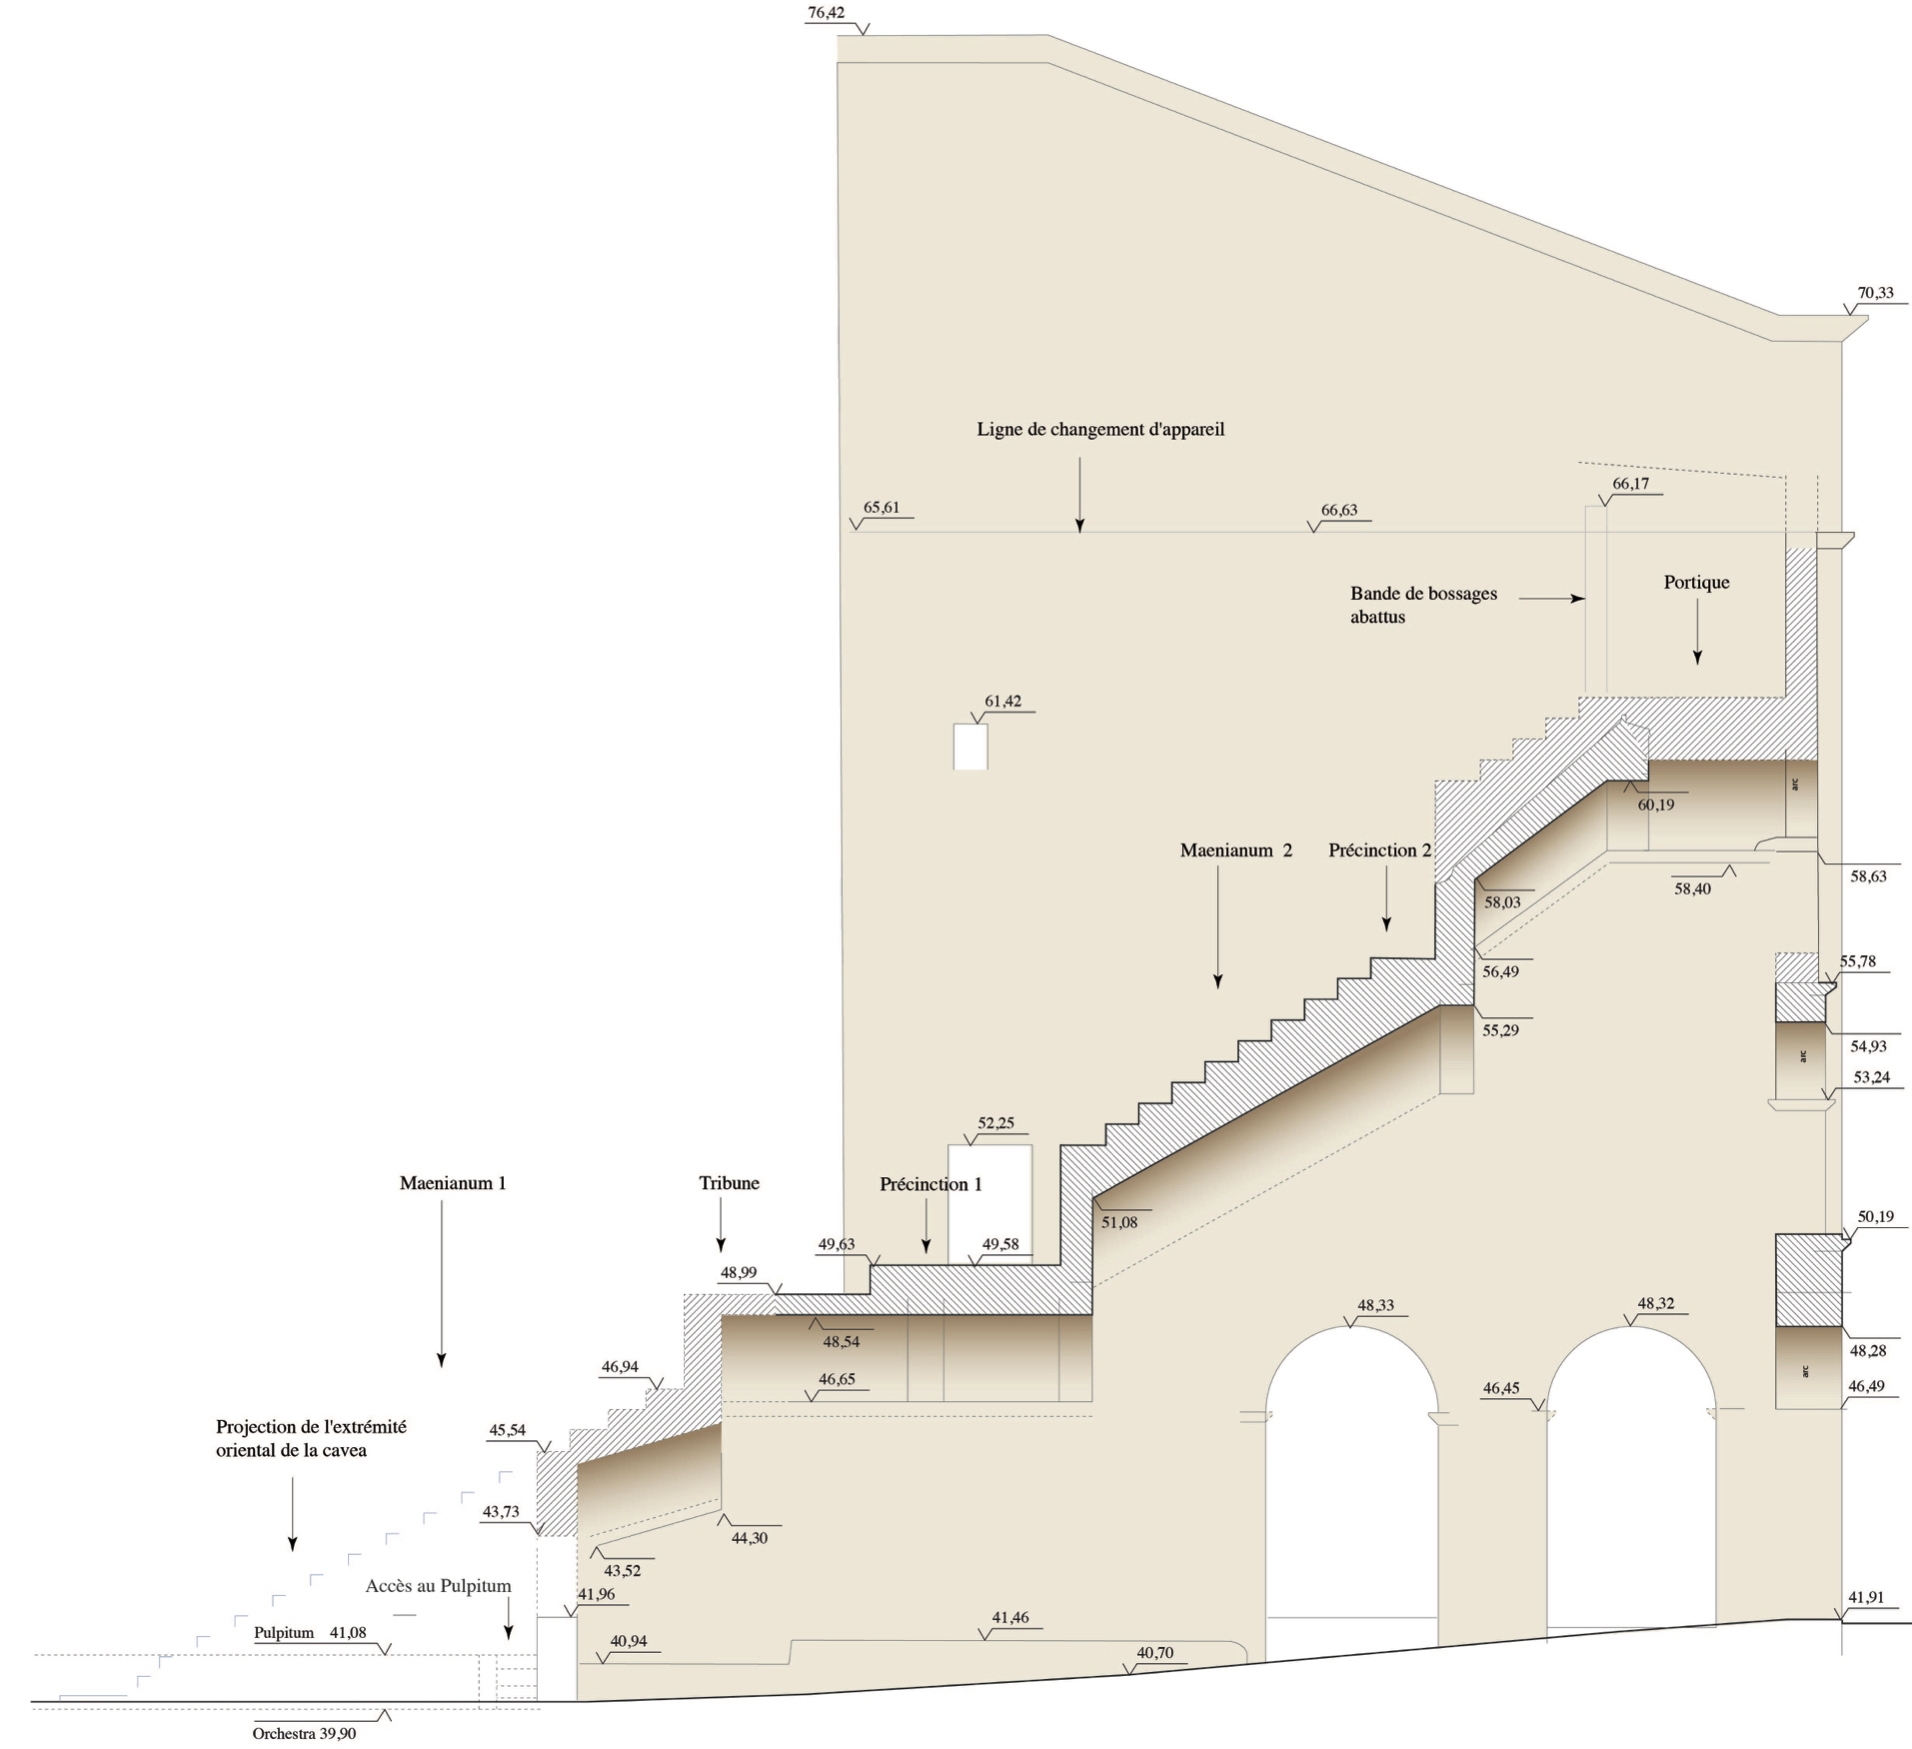
\includegraphics[width=\linewidth]{images/aditusOriental}
		\caption[Coupe sur l'\gls{aditus} oriental]{Coupe sur l'\gls{aditus} oriental \cite[Pl. XLIX]{orangePl}}
		\label{aditusOriental}
\end{figure}

\begin{figure}[!h]
	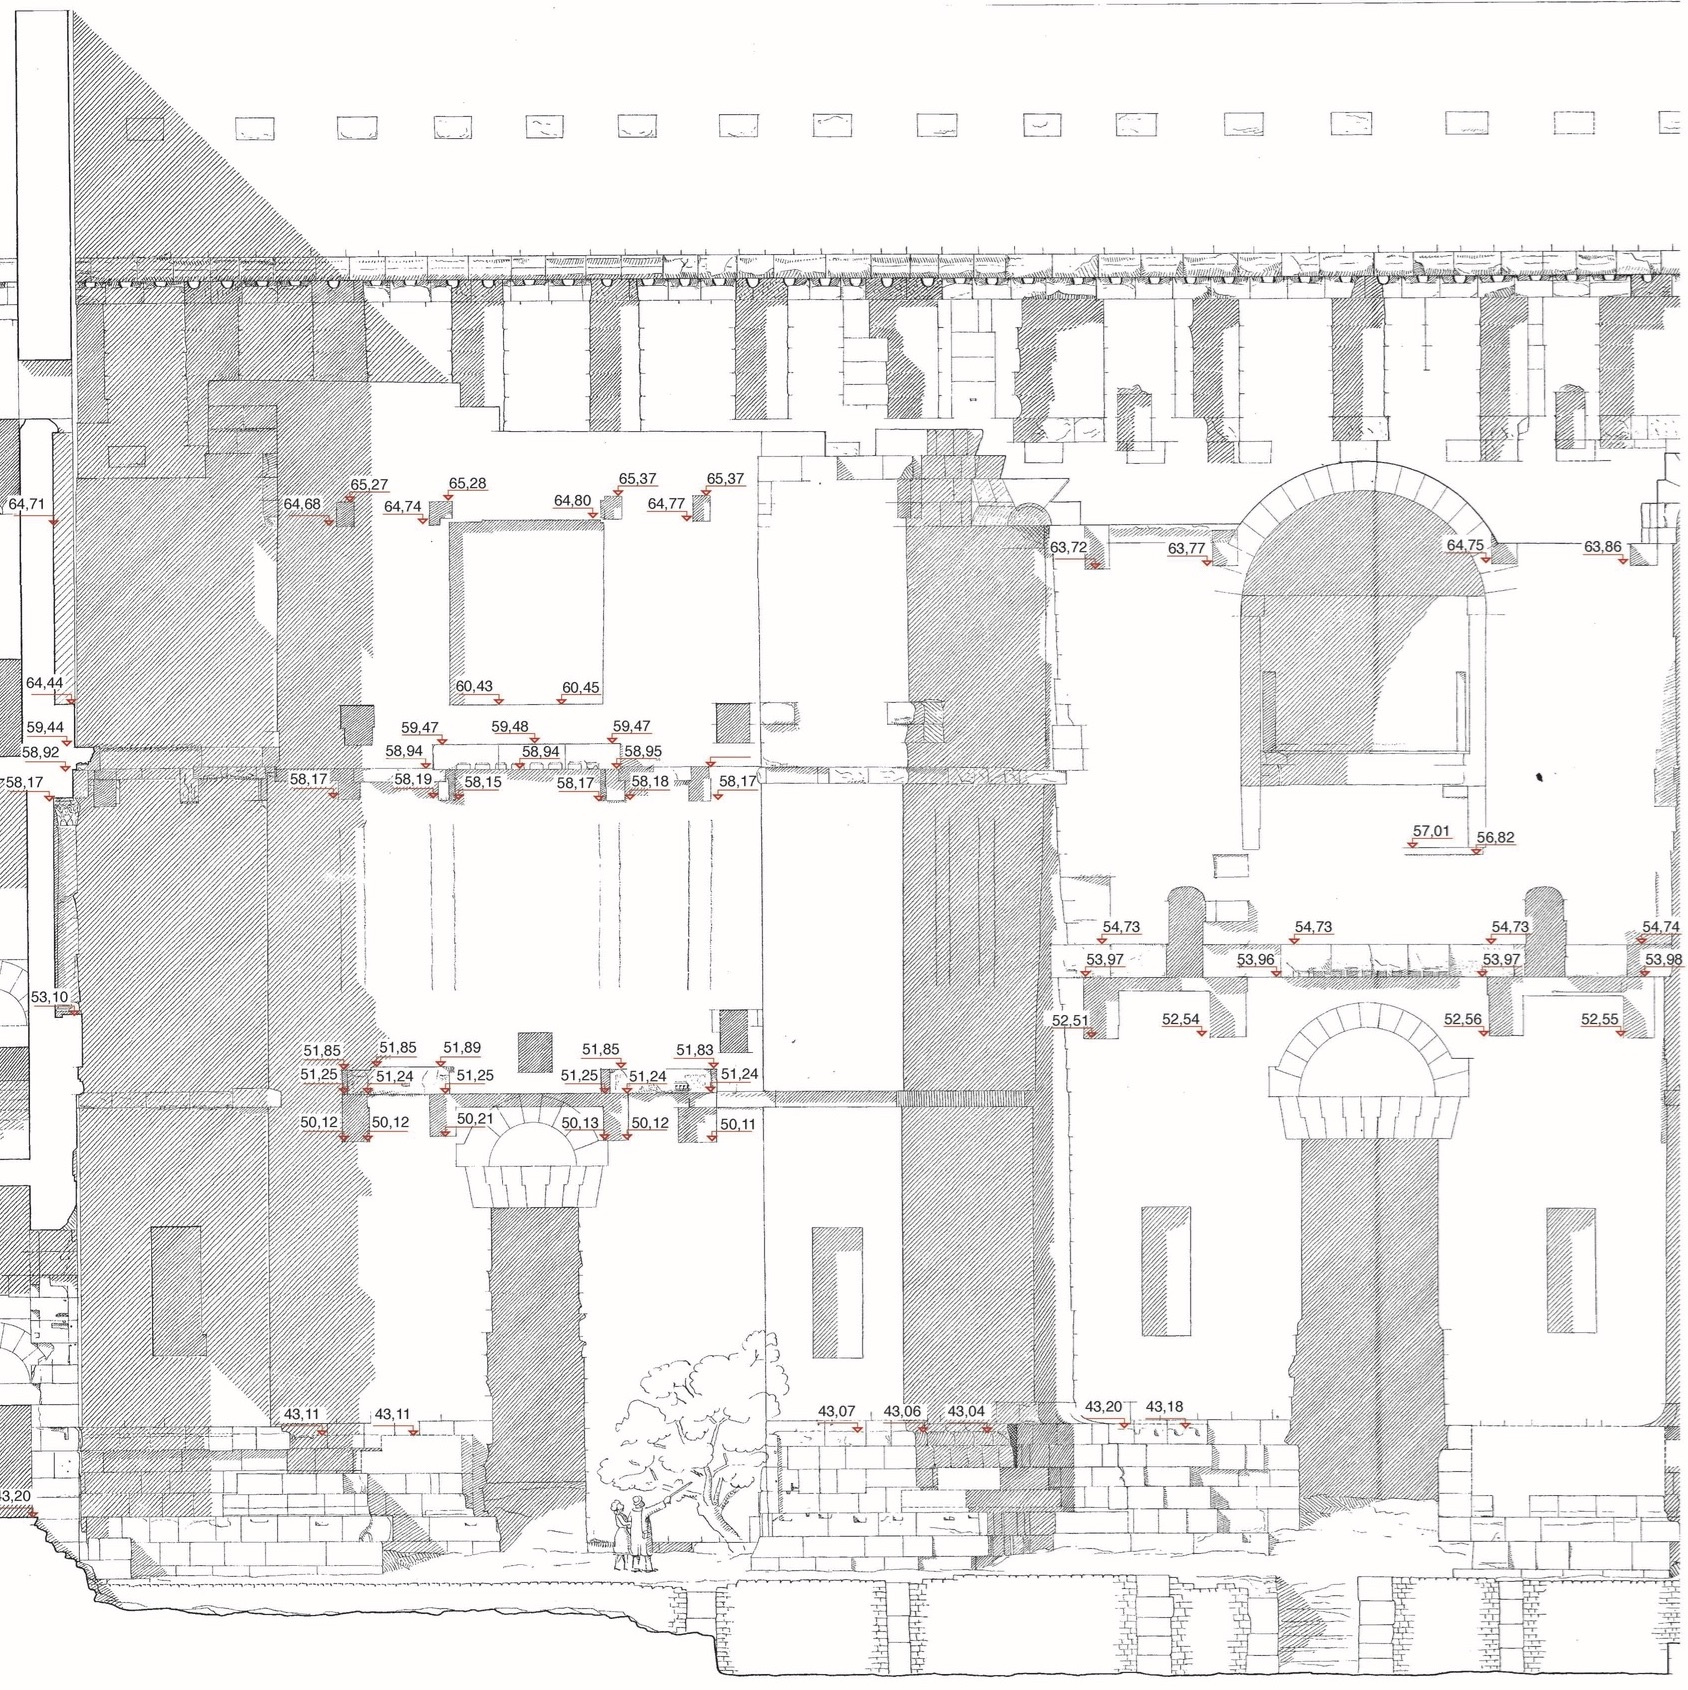
\includegraphics[width=\linewidth]{images/frontdescene}
	\caption[Elévation du front de scène]{Elévation de la partie occidentale du front de scène nivelé \cite[Pl. XXIX]{orangePl}}
	\label{frontdescene} 
\end{figure} 
	
\begin{figure}[!h]
	\includegraphics[height=0.8\paperheight]{images/retourOccidentalMur}
	\caption[Elévation du retour du mur de scène]{Elévation du retour occidental du mur de scène \cite[Pl. XXVII]{orangePl}}
	\label{retourmur} 
\end{figure} 

\begin{figure}[!h]
	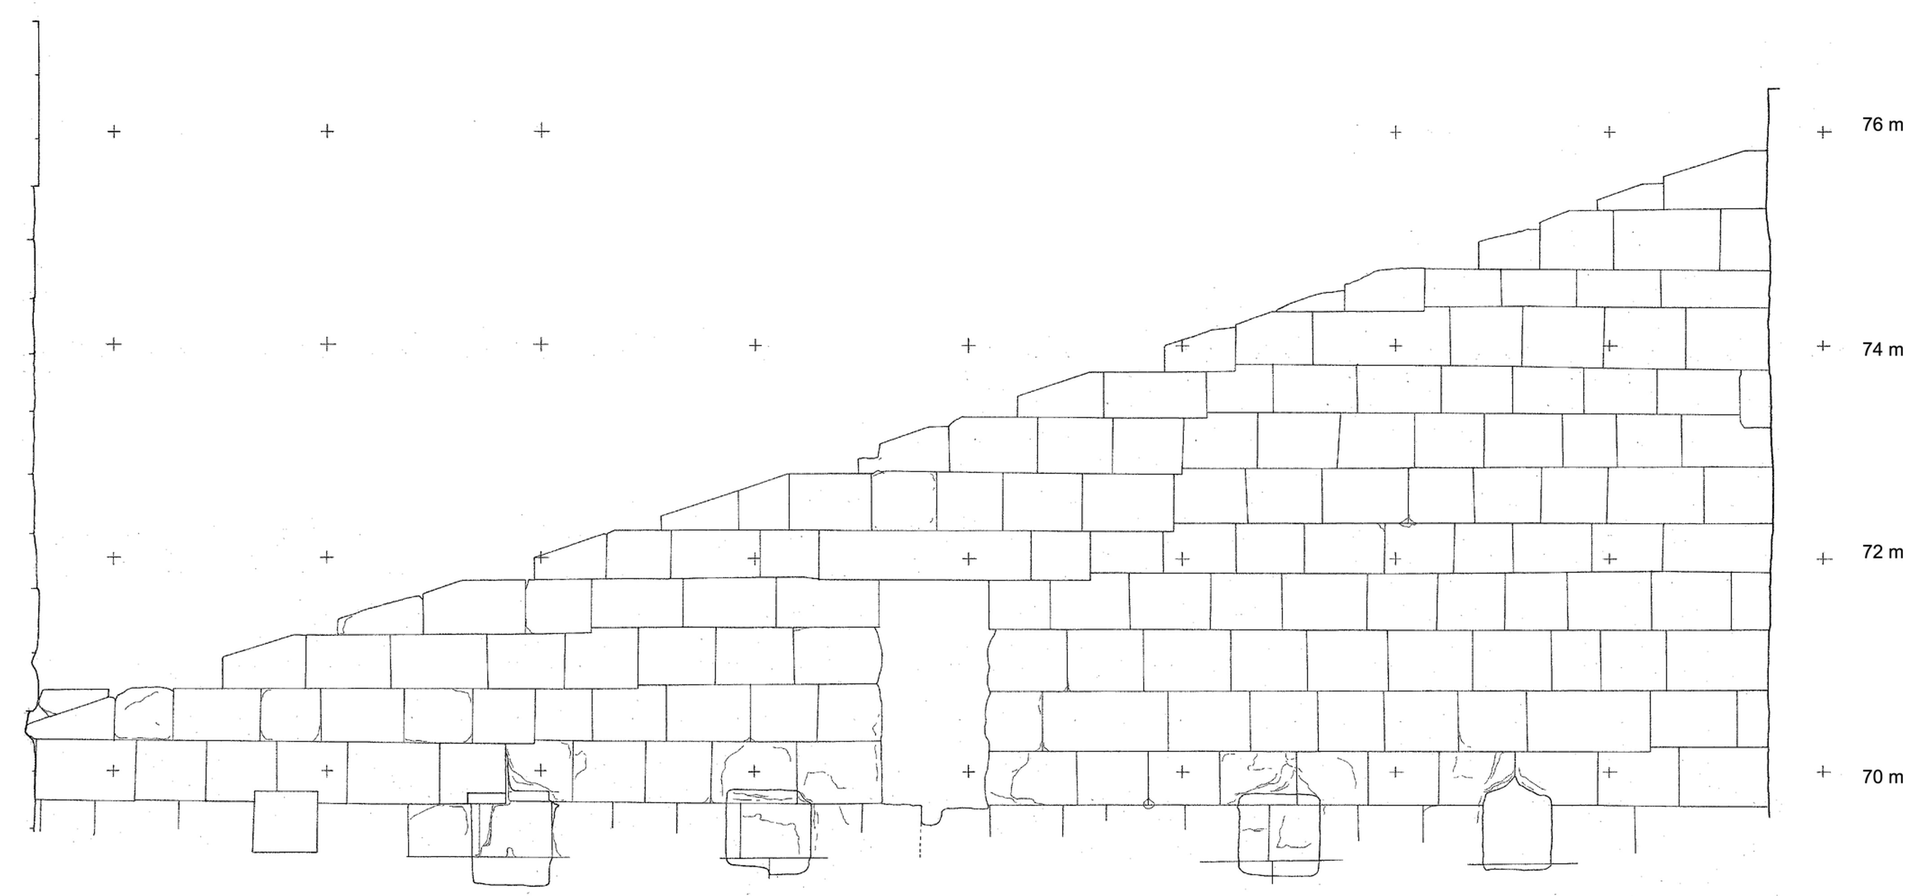
\includegraphics[width=\linewidth]{images/grenierOcci}
	\caption[Elévation de la partie sommitale de la basilique occidentale]{Elévation de la partie sommitale de la basilique occidentale \cite[Pl. XLVI]{orangePl}}
	\label{grenier} 
\end{figure} 

\begin{figure}[!h]
	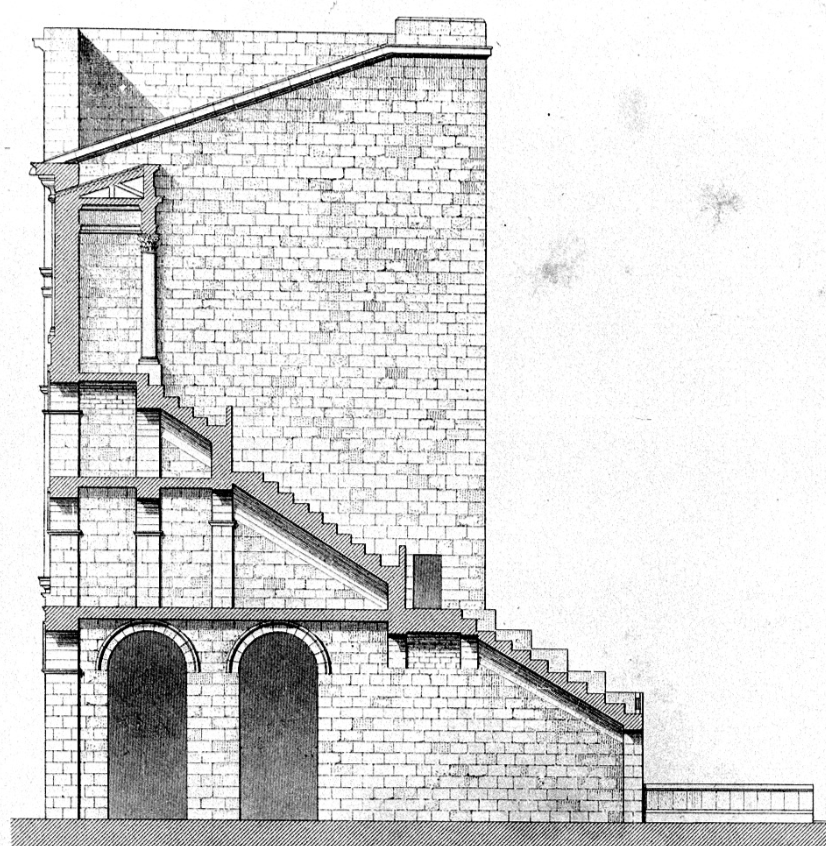
\includegraphics[width=\linewidth]{images/colonneCaristie}
	\caption[Coupe de l'\gls{aditus} occidental par A.Caristie - 1856]{Coupe de l'\gls{aditus} occidental par A.Caristie - 1856 \cite[Pl. VI]{orangePl}}
	\label{colonneCaristie} 
\end{figure}

\begin{figure}[!h]
	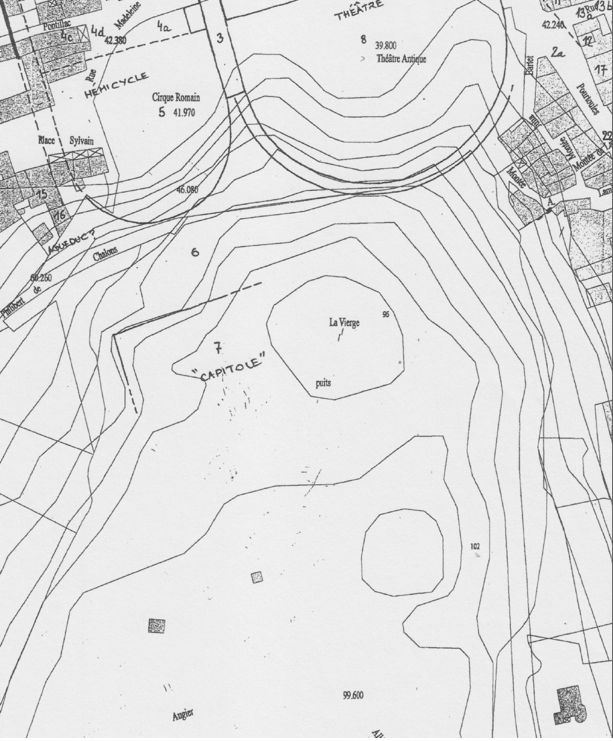
\includegraphics[width=\linewidth]{images/colline}
	\caption[Plan topographique de la colline Saint-Eutrope]{Plan topographique de la colline Saint-Eutrope \cite[p.11]{orangeTxt}}
	\label{colline} 
\end{figure} 		

\section{Tableaux annexes}

 \bibliographystyle{francaissc}
 \bibliography{Part1/Biblio}